\section{Ejercicio 2}

\subsection{Descripci\'on del problema} \label{ej_2:descripcion}

El problema se trata de un conjunto de ciudades hubicadas a cierta distancia entre ellas, las cuales todas deben de ser provistas de gas.
Para \'esto, tenemos una cantidad $k$ de centrales distribuidoras de gas, y tuber\'ias para conectar ciudades.
Una ciudad tiene gas si hay un camino de tuber\'ias que llegue hasta una central distribuidora, es decir,
si una ciudad est\'a conectada a otra ciudad por una tuber\'ia y a su vez \'esta est\'a conectada a otra ciudad
por medio de una tuber\'ia la cual tiene una central distribuidora, entonces las 3 ciudades tienen gas.
Se pide lograr que todas las ciudades tengan gas, pero que la longitud de la tuber\'ia m\'as larga de la soluci\'on
debe ser la m\'as corta posible. La longitud de una tuber\'ia es igual a la distancia entre las 2 ciudades.

El algoritmo tiene que tener una complejidad de $O(n^2)$, con $n$ la cantidad de ciudades.

De a partir de ahora, $k$ va a ser siempre la cantidad de centrales distribuidoras disponibles, y $n$ la cantidad de ciudades.

\subsubsection{Ejemplo}

Como entrada podemos tener 6 ciudades y 2 centrales distribuidoras, como en la Figura \ref{ej_2:ej:entrada}, y la soluci\'on que se busca es como indica la Figura \ref{ej_2:ej:solucion}.

\begin{figure}[htbp]
\centering
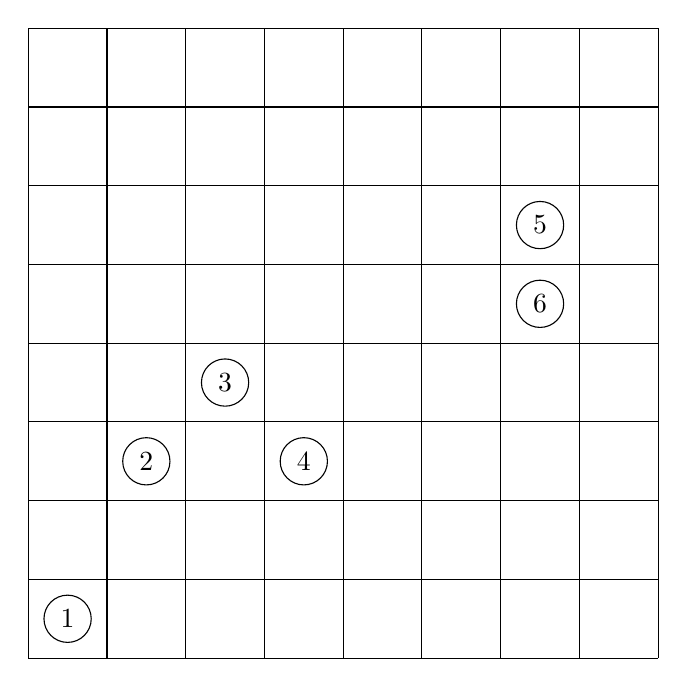
\begin{tikzpicture}

	\draw[xshift=0.5cm, yshift=0.5cm] (-1,-1) grid (7,7);
	\draw (0,0) circle [radius=0.3];
	\draw (0,0) node {1};
	\draw (1,2) circle [radius=0.3];
	\draw (1,2) node {2};
	\draw (2,3) circle [radius=0.3];
	\draw (2,3) node {3};
	\draw (3,2) circle [radius=0.3];
	\draw (3,2) node {4};
	\draw (6,5) circle [radius=0.3];
	\draw (6,5) node {5};
	\draw (6,4) circle [radius=0.3];
	\draw (6,4) node {6};
\end{tikzpicture}

\emph{Se tienen 2 centrales disponibles}

\caption{La entrada del problema, con las 5 ciudades y la cantidad de centrales}
\label{ej_2:ej:entrada}
\end{figure}

\begin{figure}[htbp]
\centering
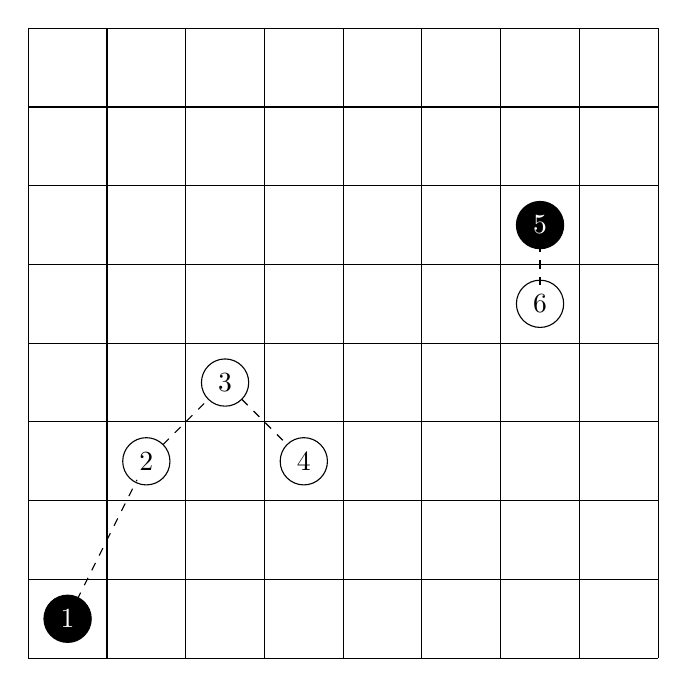
\begin{tikzpicture}
	\draw[xshift=0.5cm, yshift=0.5cm] (-1,-1) grid (7,7);
	\draw[fill=black] (0,0) circle [radius=0.3];
	\draw[white] node (v1) at (0,0) {1};
	\draw (1,2) circle [radius=0.3];
	\draw node (v2) at (1,2) {2};
	\draw[style=dashed] (v1) -- (v2);
	\draw (2,3) circle [radius=0.3];
	\draw node (v3) at (2,3) {3};
	\draw[style=dashed] (v2) -- (v3);
	\draw (3,2) circle [radius=0.3];
	\draw node (v4) at (3,2) {4};
	\draw[style=dashed] (v3) -- (v4);
	\draw[fill=black] (6,5) circle [radius=0.3];
	\draw[white] node (v5) at (6,5) {5};
	\draw (6,4) circle [radius=0.3];
	\draw node (v6) at (6,4) {6};
	\draw[style=dashed] (v5) -- (v6);
\end{tikzpicture}
\caption{La soluci\'on al problema de la Figura \ref{ej_2:ej:entrada}, los nodos negros son los que contienen las centrales de distribuci\'on}
\label{ej_2:ej:solucion}
\end{figure}


\subsection{Ideas para la resoluci\'on} \label{ej_2:idea}

Para la resoluci\'on del problema, se puede penzar en un \emph{grafo}, donde las ciudades son nodos y las tuber\'ias las aristas,
cada arista va a tener una distancia asociada que es la distancia entre los nodos (ciudades) que conecta.

Como cada ciudad tiene gas si hay un camino hasta una central distribuidora, entonces todas las ciudades que se conectan
a una misma central pertenecen a una misma componente conexa. Como tenemos un m\'aximo de $k$ centrales, la soluci\'on tiene que tener un m\'aximo de $k$ componentes conexas y las centrales se colocar\'an cada una en una componente conexa y en cualquier ciudad dentro de la componente conexa, ya que la distancia de las aristas dentro de una componente conexa no se ver\'a modificada si se cambia de nodo la central dentro de la misma componente conexa.

Entonces, la soluci\'on que se pide es que el grafo tenga a lo sumo $k$ componentes conexas, y que la distancia de la arista mas larga, sea la m\'as corta posible.

Una idea que se propone es comenzar con todos los nodos sueltos, sin ninguna arista conectada,
y calcular todas las distancias entre todos los nodos, es decir, calcular todas las tuber\'ias posibles con sus respectivas distancias.
Luego se ordenar\'an las aristas (tuber\'ias) de menor a mayor de acuerdo a sus longitudes.
Se calcula si la cantidad de componentes conexas es menor o igual a $k$, si es as\'i, entonces el algoritmo termina, sino coloca la tuber\'ia m\'as corta que no genere un ciclo y contin\'ua preguntando sobre la cantidad de componentes conexas e iterando sobre las aristas siguiendo el orden de menor a mayor.
B\'asicamente es aplicar \emph{Kruskal} sobre un grafo completo.

Como se requiere tener todas las aristas ordenadas por peso, en un grafo completo tenemos $n(n-1)/2$ aristas, dandonos una complejidad de al menos $O(n^2 \log n^2)$, y no cumple con el requerimiento.
Para mejorar la complejidad del algoritmo, en vez de calcular la distancia de todos las aristas e iterar sobre todas las aristas, requiriendo ordenar por peso \emph{todas} las aristas, primero creamos un \'arbol generador m\'inimo (con las aristas m\'as cortas posibles), con una idea como el algoritmo de \emph{Prim} y que tenga de cota $O(n^2)$,
el \'arbol generador m\'inimo generado nos queda $n - 1$ aristas, y luego, al igual que antes, se ordenan y se recorren esas $n - 1$ aristas de menor a mayor.

En resumen, la idea es partir de un grafo completo con $n$ nodos, aplicar \emph{Prim} y obtener el \emph{AGM}, luego sobre ese \'arbol aplicar \emph{Kruskal} pero cortando el algoritmo cuando se tienen tantas componentes conexas como $k$ centrales de gas. La colocaci\'on de las centrales de gas se colocan luego en un nodo cualquiera de los nodos de cada componente conexa.

En la secci\'on \ref{ej_2:algoritmo} se propone un pseudoc\'odigo, en la secci\'on \ref{ej_2:ejemplo} se ver\'a un ejemplo de ejecuci\'on del algoritmo,
en la secci\'on \ref{ej_2:justificacion} se justificar\'a la correctitud, y en la secci\'on \ref{ej_2:cota} se har\'a el c\'alculo de la complejidad del algoritmo.

\subsubsection{Algoritmo} \label{ej_2:algoritmo}

\begin{algorithm}[!h]
\caption{minimizarTuberias} \label{ej_2:pseudo}
\end{algorithm}
\begin{algorithmic}[1]
	\Require \emph{centrales}: cantidad de centrales disponibles, mayor que 0
	\Require \emph{ciudades}: las ciudades con sus posiciones
	\Require \emph{n}: cantidad de ciudades en el par\'ametro \emph{ciudades}
	\Statex
	\Ensure Retorna el grafo tal que hay tanas componentes conexas como \emph{centrales}, y que la arista m\'as larga es la m\'as corta posible
	\Statex
	\Procedure{minimizarTuberias}{Entero: centrales, Array: ciudades, Entero: n}{$\to$ Grafo}
		\State Grafo g $\gets$ \Call{NuevoGrafo}{$n$} \Comment{Creo un grafo con $n$ nodos, sin aristas}
		\State $<$bool agregado, entero distancia, entero nodo$>$  nodos[n] \Comment{La distancia es desde $n$ (\'indice del array) hasta nodos[$n$].nodo}
		\State $<$nodo1, nodo2, distancia$>$ aristas[n - 1]
		\Statex
		\State nodos[0] $\gets$ $<$true, 0, 0$>$ \label{ej_2:pseudo:inicializa}
		\For{i $\gets$ 1; i $<$ n; i$++$} \label{ej_2:pseudo:distancia}
			\State nodos[i] $\gets$ $<$false, \Call{Distancia}{ciudades[i], ciudades[0]}, 0$>$
		\EndFor \label{ej_2:pseudo:fin_inicializa}
		\Statex
		\For{agregados $\gets$ 0; agregados $<$ n - 1; agregados$++$} \label{ej_2:pseudo:crea_arbol}
			\State distancia\_minima $\gets$ $\infty$
			\State nodo\_minimo $\gets$ 0
			\For{i $\gets$ 0; i $<$ n; i$++$} \Comment{Busco el nodo mas cercano al \'arbol que ya tenemos} \label{ej_2:pseudo:mas_cerca}
				\If{nodos[i].agregado = false}
					\If{nodos[i].distancia $<$ distancia\_minima}
						\State distancia\_minima $\gets$ nodos[i].distancia
						\State nodo\_minimo $\gets$ i
					\EndIf
				\EndIf
			\EndFor \label{ej_2:pseudo:fin_mas_cerca}
			\Statex
			\State nodos[nodo\_minimo].agregado $\gets$ true \label{ej_2:pseudo:nodo}
			\State aristas[agregados] $\gets$ $<$nodo\_minimo, nodo[nodo\_minimo].nodo, distancia\_minima$>$ \Comment{Agrego el nodo encontrado} \label{ej_2:pseudo:arista}
			\Statex
			\For{i $\gets$ 0; i $<$ n; i$++$} \Comment{Actualizo la distancia de los nodos no agregados a\'un} \label{ej_2:pseudo:actualiza}
				\If{nodos[i].agregado = false}
					\If{nodos[i].distancia $>$ \Call{Distancia}{ciudades[i], ciudades[nodo\_minimo]}}
						\State nodo[i].distancia $\gets$ \Call{Distancia}{ciudades[i], ciudades[nodo\_minimo}
						\State nodo[i].nodo $\gets$ nodo\_minimo
					\EndIf
				\EndIf
			\EndFor \label{ej_2:pseudo:fin_actualiza}
		\EndFor \label{ej_2:pseudo:fin_crea_arbol}
		\Statex
		\State \Call{Ordenar}{aristas} \Comment{Ordeno las aristas por la distancia} \label{ej_2:pseudo:sort}
		\Statex
		\For{componentes $\gets$ n; componentes $>$ centrales; componentes$--$} \label{ej_2:pseudo:componentes}
			\State \Call{AgregarArista}{g, aristas[n - componentes].nodo1, aristas[n - componentes].nodo2}
		\EndFor \label{ej_2:pseudo:fin_componentes}
		\State retornar $\gets$ g
	\EndProcedure
\end{algorithmic}



\subsubsection{Ejemplo de ejecuci\'on} \label{ej_2:ejemplo}

\subsection{Justificaci\'on del procedimiento} \label{ej_2:justificacion}

Para la justificaci\'on vamos a justificar primero que si se aplica el algoritmo de \emph{Kruskal} sobre el \emph{AGM} generado por el algoritmo de \emph{Prim} dado un grafo completo, entonces llegamos a un grafo con pesos de aristas iguales que aplicar \emph{Kruskal} sobre el grafo completo directamente, aunque puede tener aristas diferentes de igual peso. Como tienen los mismos pesos aunque las arisas sean diferentes, a efectos de minimizar el peso de la arista de mayor peso da el mismo resultado. (Secci\'on \ref{ej_2:demo:k}).

Luego vamos a justificar que aplicando el algoritmo de \emph{Kruskal} sobre un grafo completo pero cortando cuando tenemos $K$ componentes conexas, nos genera la soluci\'on que buscamos (Secci\'on \ref{ej_2:demo:p}).

Teniendo demostrado esos 2 puntos, entonces aplicar \emph{Kruskal} a un grafo completo nos da la soluci\'on que buscamos y aplicar \emph{Kruskal} al resultado \emph{Prim} (que es lo que realiza el algoritmo propuesto) nos da el mismo resultado que aplicar \emph{Kruskal} directamente, siendo la soluci\'on buscada.

\subsubsection{Demostraci\'on de Kruskal sobre Prim} \label{ej_2:demo:k}

Demostraremos que aplicar el algoritmo de \emph{Kruskal} sobre un grafo completo da aristas con los mismos pesos que aplicar \emph{Kruskal} sobre el \emph{AGM} resultante del algoritmo de \emph{Prim}. Como el problema pone restricci\'on sobre el peso de las aristas (de las tuber\'ias), entonces nos fijaremos que las aristas del resultado pueden ser diferentes pero si se mira s\'olo los pesos de las aristas, estos son los mismos.

\begin{proof}
	Un \emph{AGM} de un grafo tiene como suma de los pesos de sus aristas, la menor suma posible de todos los \'arboles de un grafo. Si se aplica \emph{Prim} y \emph{Kruskal} a un mismo grafo (un grafo completo por ejemplo), ambos dan un \emph{AGM} como resultado, por ende el peso del \'arbol generado por \emph{Prim} del grafo g ($P_p(g)$) es igual al peso del que genera \emph{Kruskal} ($P_k(g)$), si no fueran iguales, el que tiene mayor peso no ser\'ia un \emph{AGM}. Como \'ambos son \'arboles del mismo grafo, ambos tienen $n-1$ aristas ($n = $ cantidad de nodos del grafo).

	\begin{equation*}
	\begin{split}
		P_p(g) = \sum_{i = 0}^{i < n - 1} \pi(a_i)\\
		=\\
		P_k(g) = \sum_{i = 0}^{i < n - 1} \pi(a_i)
	\end{split}
	\end{equation*}

Como \emph{Prim} y \emph{Kruskal} son 2 algoritmos diferentes, podr\'ian generar un \'arbol con diferentes aristas pero igual mantienen la igualdad en la suma de los pesos y la cantidad de aristas.

Supongamos que un algoritmo pone las mismas aristas que el otro pero en vez de poner la arista $a$ pone la arista $a'$ con distinto peso, entonces tambi\'en tiene que haber cambiado otra arista $b$ por $b'$ para mantener la igualdad de la suma. Supongamos que tenemos todas las aristas $a_i$ del \emph{AGM} y las ordenamos de menor a mayor y de la arista $a_0$ a $a_{j-1}$ y de $a_j+2$ a $a_{n-2}$ las aristas son las mmismas para ambos algoritmos pero $a_j$ y $a_{j+2}$ son diferentes, entonces:

	\begin{equation*}
	\begin{split}
		P_p(g) = \sum_{i = 0}^{i < j} \pi(a_i) + \pi(a') + \pi(b') + \sum_{i = j + 2}^{i < n - 1} \pi(a_i) \\
		=\\
		P_k(g) = \sum_{i = 0}^{i < j} \pi(a_i) + \pi(a) + \pi(b) + \sum_{i = j + 2}^{i < n - 1} \pi(a_i)
	\end{split}
	\end{equation*}

Simplificamos la igualdad de las suma, nos queda:

	\begin{equation*}
	\begin{split}
		\pi(a') + \pi(b') \\
		=\\
		\pi(a) + \pi(b)
	\end{split}
	\end{equation*}

	Como dijimos que el peso de $a'$ es distinto de $a$, podemos suponer que $\pi(a) > \pi(a')$ y por lo tanto $\pi(b) < \pi(b')$ (se puede suponer tambi\'en lo contrario y ser\'ia an\'alogo). \emph{Prim} entonces hubiera agregado $a'$ con menor peso que $a$, pero como \emph{Kruskal} recorre las aristas de menor a mayor peso, ya tendr\'ia que haber pasado por $a'$, y como las aristas anteriores a $a'$ son las mismas en ambos algoritmos, agregar $a'$ no genera ciclos, entonces \emph{Kruskal} hubiera agregado a $a'$, entonces $\pi(a') = \pi(a)$ porque $a' = a$. A\'un quedar\'ia $\pi(b') \neq \pi(b)$, pero como todas las dem\'as aristas son las mismas (incluidas $a'$ y $a$), entonces para mantener la igualdad de la suma $\pi(b') = \pi(b)$, contradiciendo la suposci\'on que un algoritmo cambiaria una arista por otra con peso dinstinto.

	Si cambia una arista por otra de igual peso, no modifica la soluci\'on porque el peso de la arista de mayor peso seguir\'ia siendo el mismo.

	Como aplicar \emph{Kruskal} a un \'arbol da el mismo \'arbol (porque es el \'unico subgrafo que es un \'arbol), aplicar \emph{Kruskal} al resultado de \emph{Prim} da el mismo resultado que aplicar directamente \emph{Prim}, y ya demostramos que aplicar \emph{Prim} y \emph{Kruskal} dan \'arboles con mismos pesos de aristas, por lo que aplicar \emph{Kruskal} directamente o aplicar \emph{Kruskal} a la salida de \emph{Prim}, da \'arboles con los mismos pesos de aristas.

\end{proof}

\subsubsection{Demostraci\'on de que aplicar Kruskal nos genera la soluci\'on} \label{ej_2:demo:p}

Demostraremos que teniendo un grafo completo, si aplicamos \emph{Kruskal} y dejamos de agregar aristas cuando llegamos a $k$ componentes conzas, tenemos la soluci\'on que buscamos:

\begin{proof}
	El algoritmo de \emph{Kruskal} ordena las aristas de menor a mayor seg\'un su peso, y agrega 1 a 1 las aristas seg\'un dicho orden tal que no genere un ciclo. Al agregar una arista se disminuye en 1.  Nosotros detendremos el algoritmo cuando se llego a $k$ componentes conezas.
	Supongamos que tenemos $m$ aristas ordenadas de menor a mayor por su peso, ($a_0, a_1 .. a_i .. a_{m-1}$), que se fueron agregando (aunque algunas generaban ciclos y no se agregaron), y que detuvimos el algoritmo de \emph{Kruskal} al agregar la arista $a_j$ porque se llegaron a $k$ componentes conexas. Entonces, como las aristas estaban ordenadas:
	\begin{equation*}
	\begin{split}
		(\forall 0 \leq i < j) a_i \leq a_j \\
		\land \\
		(\forall j < i < m) a_i \geq a_j \\
	\end{split}
	\end{equation*}
	Todos los $a_i, i < j$ est\'an agregados al resultado de \emph{Kruskal}.

	El $a_j$ es la arista de mayor peso (la tuber\'ia m\'as larga), y es la que queremos minimiza.

	Si existiese una mejor forma de armar las componentes conexas, entonces existe un $a_i, a_i < a_j \implies i < j$, tal que se puede reemplazar $a_i$ por $a_j$ y as\'i terner la arista de mayor peso que es de menor peso que la que obtuvimos. Como $i < j$, \emph{Kruskal} ya la analiz\'o $a_i$ antes de pasar por $a_j$.

	Si $a_i$ no generaba ciclos, entonces esa arista pertenece al resultado del algoritmo, y como no se detuvo en $a_i$ significa que a\'un agregando esa arista (y todas las anteriores) no se llegaban a las $k$ componentes componentes conexas que se buscan, entonces no se puede sacar $a_j$ porque no se llegar\'ia a la cantidad de componentes conexas necesarias, contradiciendo que se puede quitar $a_j$ para mejorar la soluci\'on.

	Si $a_i$ generaba un ciclo, entonces esa arista no pertenece al resultado del algoritmo. Notar que como $a_i$ se analiza antes que $a_j$ por tener menor peso, entonces $a_i$ generaba un ciclo cuando $a_j$ a\'un no estaba agregada. Si se quita $a_j$ y se agrega $a_i$, al quitar $a_j$ se aumenta en 1 la cantidad de componentes conexas (ahora tenemos $k + 1$) y no es soluci\'on, y al agregar $a_i$ se est\'a generando un ciclo, por lo que no disminuye la cantidad de componentes conexas, manteniendose en $k + 1$ y no es soluci\'on tampoco, por lo que contradice que se puede quitar $a_j$ para agregar $a_i$ y tener una mejor soluci\'on.

	Entonces, agregar aristas en orden seg\'un su peso si no genera ciclos y parar cuando se alcanzan las $k$ componentes conexas, nos da como peso de la arista m\'as larga, el peso mas chico posible, siendo la soluci\'on que se busca del problema.

\end{proof}

\subsection{Cota de complejidad} \label{ej_2:cota}

Se analiza la complejidad de algoritmo \ref{ej_2:pseudo}, para \'esto se supone que el c\'alculo de la distancia entre ciudades (el peso de las aristas/tuber\'ias) se realiza en $O(1)$

La cantidad de nodos se representar\'a como $n$, y la cantidad de centrales como $k$.

\begin{itemize}
	\item La inicializaci\'on de unas variables se realiza de la l\'inea \ref{ej_2:pseudo:inicializa} a \ref{ej_2:pseudo:fin_inicializa}, y se realizan $n$ iteraciones calculando la distancia y guardando en un vector, quedando $O(n)$
	\item Para la creaci\'on del AGM entre las l\'ineas \ref{ej_2:pseudo:crea_arbol} a \ref{ej_2:pseudo:fin_crea_arbol} realiza $n - 1$ iteraciones
	\begin{itemize}
		\item L\'ineas \ref{ej_2:pseudo:mas_cerca} a \ref{ej_2:pseudo:fin_mas_cerca}, busca el nodo m\'as cercano, realizando $n$ iteraciones de comparaciones y asignaciones que son $O(1)$, quedandonos $O(n)$
		\item Las l\'ineas \ref{ej_2:pseudo:nodo} y \ref{ej_2:pseudo:arista} son $O(1)$
		\item La actualizaci\'on de las distancias, entre las l\'ineas \ref{ej_2:pseudo:actualiza} y \ref{ej_2:pseudo:fin_actualiza} realiza $n$ iteraciones de comparaciones y asignaciones que son $O(1)$, quedandonos $O(n)$
	\end{itemize}
	\item Ordenar las aristas en la l\'inea \ref{ej_2:pseudo:sort}, y se realizan sobre las aristas agregadas en la iteraci\'on anterior, la cual agrega $n-1$ aristas, entonces se ordenan $n - 1$ elementos. Al $n$ no estar acotado, se puede realizar con algoritmos como \emph{MergeSort} o \emph{HeapSort} en $O(n \log n)$
	\item Entre las l\'ineas \ref{ej_2:pseudo:componentes} y \ref{ej_2:pseudo:fin_componentes} se realizan $n - k$ iteraciones, implementando el grafo \emph{g} en una \emph{matriz de adyacencia}, \emph{AgregarArista} se realiza en $O(1)$, quedandonos una complejidad de $O(n - k)$. Notar que si $k > n$, no se realiza ninguna iteraci\'on.
\end{itemize}

Bajo \'este an\'alisis, la complejidad nos queda (\ref{ej_2:cota:formula})

\begin{equation}
\label{ej_2:cota:formula}
\begin{split}
O(n) + (n-1)*(O(n) + O(1) + O(n)) + O(n \log n) + O(n - k) \\
=
O(n) + O(n^2) + O(n) + O(n^2) + O(n \log n) + O(n - k) \\
=
O(2n) + O(2n^2) + O(n \log n) + O(n - k) \\
= O(n^2)
\end{split}
\end{equation}

Cumpliendo as\'i la complejidad requerida.

\subsection{Casos de prueba y resultado del programa} \label{ej_2:casos}

\subsection{Mediciones de performance} \label{ej_2:performance}

\subsection{Concluciones} \label{ej_2:concluciones}

